\section{Experimental Results}
\label{sec:pmc-results}

This chapter presents the results of predicting memory consumption from seismic input shapes.
The results are evaluated into five main categories: (i) memory and execution-time profiling, (ii) model performance overview, (iii) feature selection experiments, (iv) data reduction studies, and (v) cross-operator comparisons.
Each section provides insights into the memory usage patterns of the seismic operators, the performance of regression models, the impact of feature selection, and the robustness of the models under data scarcity.
All analyses and experiment results are located in the \texttt{experiment} directory of the project repository~\cite{delucca2025experiment2results}.

\subsection{Experiment Outputs Overview}
\label{subsec:pmc-results-experiment-outputs-overview}

This section introduces the operators under study, highlights the main experimental goals, and outlines key data artifacts.
The final segments of the pipeline generated five distinct \ac{CSV} files that consolidate memory usage measurements, model evaluations, feature selection outcomes, and data-reduction experiments.
These artifacts form the basis for subsequent analyses in the following sections.

\vspace{1em}
\noindent
\textbf{Operators and Experimental Goals.}
Three operators were evaluated: Envelope, \ac{GST3D}, and the 3D Gaussian Filter.
All three process seismic data volumes and exhibit distinct computational traits.
The primary objective involved modeling their peak \ac{RAM} consumption based on shape parameters (inlines, xlines, and samples), thereby enabling more informed \ac{HPC} resource allocations.

\vspace{1em}
\noindent
\textbf{Data Artifacts.}
The experiment produced five core \ac{CSV} files:
\begin{enumerate}
    \item \emph{profile\_history.csv}:
    Time-series snapshots of \ac{RSS} and corresponding timestamps.
    Each row represents one data capture during an operator’s execution.
    \item \emph{profile\_summary.csv}:
    Aggregated statistics about peak memory usage and execution time per input volume.
    This file stores the mean, standard deviation, minimum, and maximum peak memory usage, along with average runtimes and related descriptors.
    \item \emph{model\_metrics.csv}:
    Performance metrics (\ac{RMSE}, \ac{MAE}, $R^2$, accuracy, and an overall score) for each trained regression model.
    It also includes arrays of residuals, predicted values, and ground truths for deeper error analysis.
    \item \emph{feature\_selection.csv}:
    Results of experiments that use different subsets of features to predict memory usage.
    Each row documents the selected features, model configuration, and associated performance (\ac{RMSE}, \ac{MAE}, $R^2$, accuracy, and score).
    \item \emph{data\_reduction.csv}:
    Outputs from varying the number of training samples.
    The file compares performance metrics across multiple training-set sizes to study model robustness under data scarcity.
\end{enumerate}

\vspace{1em}
\noindent
\textbf{Shape Configurations.}
The synthetic datasets spanned multiple \ac{3D} dimensions.
Volumes ranged from smaller shapes (e.g., $100$ $\times$ $100$ $\times$ $100$) to significantly larger ones close to memory limits of the test system.
Each operator was executed for these volumes to capture comprehensive memory-profiling data.
This systematic approach reveals how memory usage and execution time evolve as the number of traces or samples grows.

\vspace{1em}
\noindent
\textbf{Chapter Roadmap.}
Section~\ref{sec:pmc-results-memory-and-execution-time-profiling} first presents how memory usage behaved during operator runs and highlights the aggregated profiling statistics.
Subsequent sections detail model performance across regression approaches, emphasizing how different features and training subsets affect accuracy.
The final portion compares Envelope, \ac{GST3D}, and Gaussian Filter side by side to underscore differences and provide practical insights for \ac{HPC} scheduling.


\section{Memory and Execution-Time Profiling}
\label{sec:pmc-results-memory-and-execution-time-profiling}

This section examines how memory usage and execution time scale with input volume and seismic dimension sizes for Envelope, \ac{GST3D}, and the Gaussian Filter.

\subsection{Linear Trends and Variability}
\label{subsec:linear-trends-and-variability}

Figure~\ref{fig:peak_memory_facet} show that average peak memory usage grows linearly with increasing volume for Envelope, \ac{GST3D}, and Gaussian Filter.
A higher \ac{CV} is observed for smaller volumes, whereas larger volumes yield more stable, yet higher, memory consumption.

\begin{figure*}[htbp]
    \centering
    \begin{subfigure}[t]{0.49\textwidth}
        \centering
        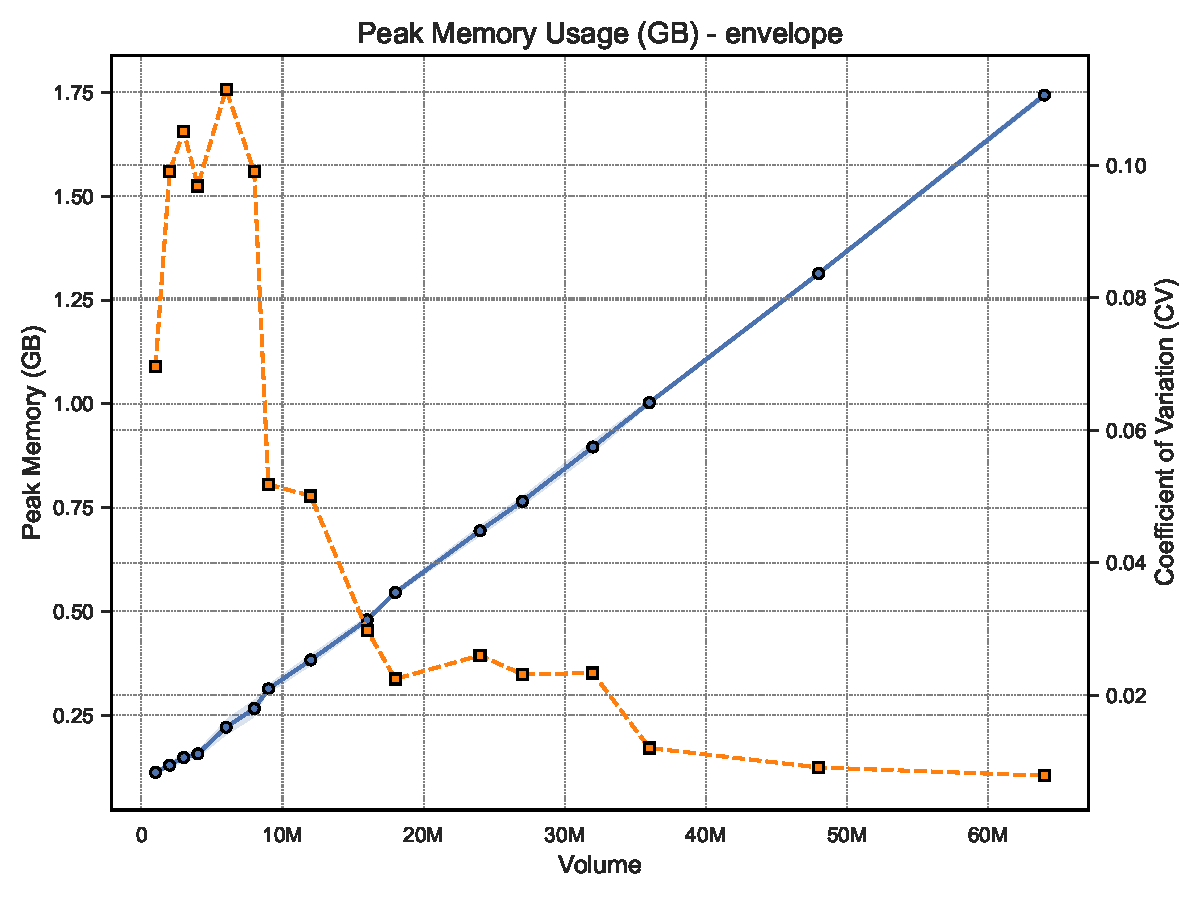
\includegraphics[width=\textwidth]{assets/images/05/peak_memory_by_volume_envelope}
        \caption{Envelope: Smaller volumes exhibit higher variability,
            while larger volumes show a consistent linear growth.}
    \end{subfigure}
    \hfill
    \begin{subfigure}[t]{0.49\textwidth}
        \centering
        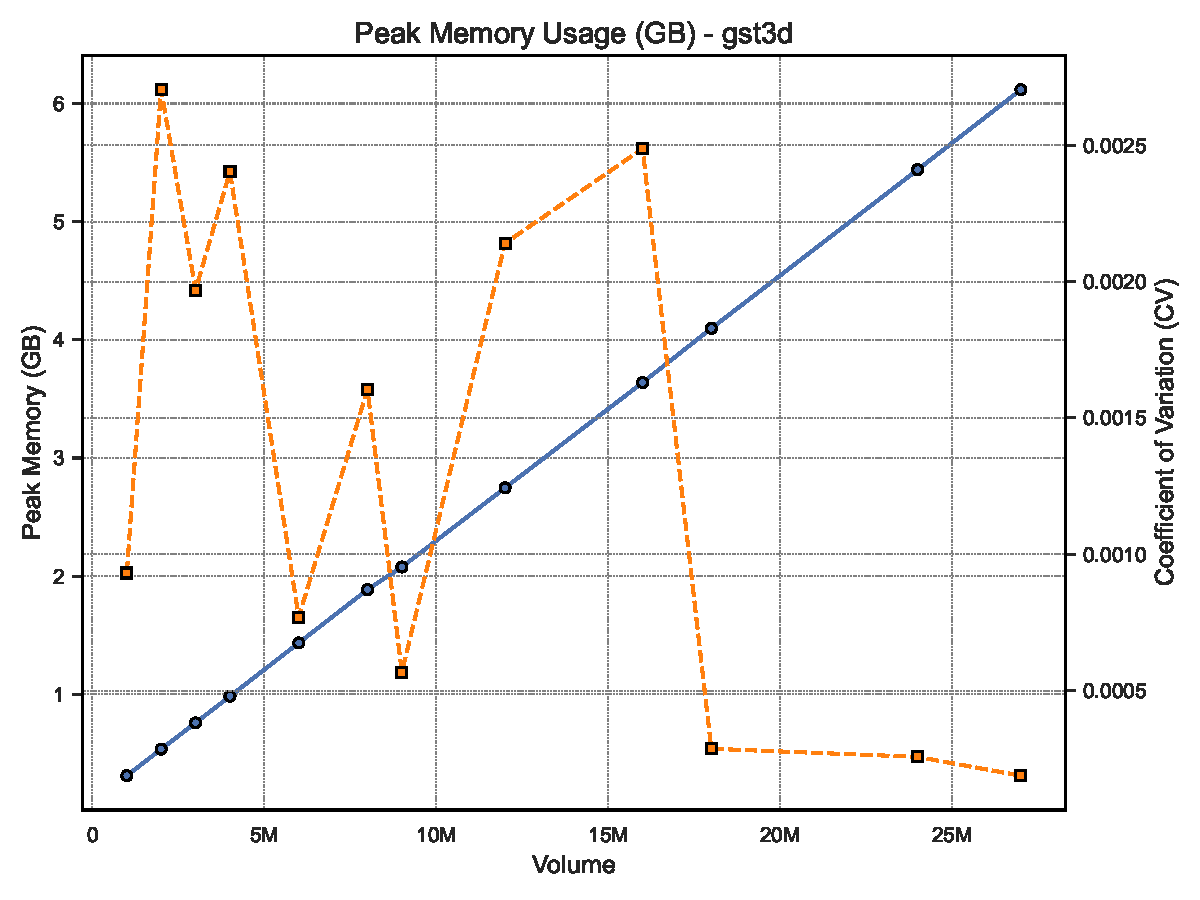
\includegraphics[width=\textwidth]{assets/images/05/peak_memory_by_volume_gst3d}
        \caption{\ac{GST3D}: Exhibits a steeper slope relative to Envelope.}
    \end{subfigure}
    \hfill
    \begin{subfigure}[t]{0.49\textwidth}
        \centering
        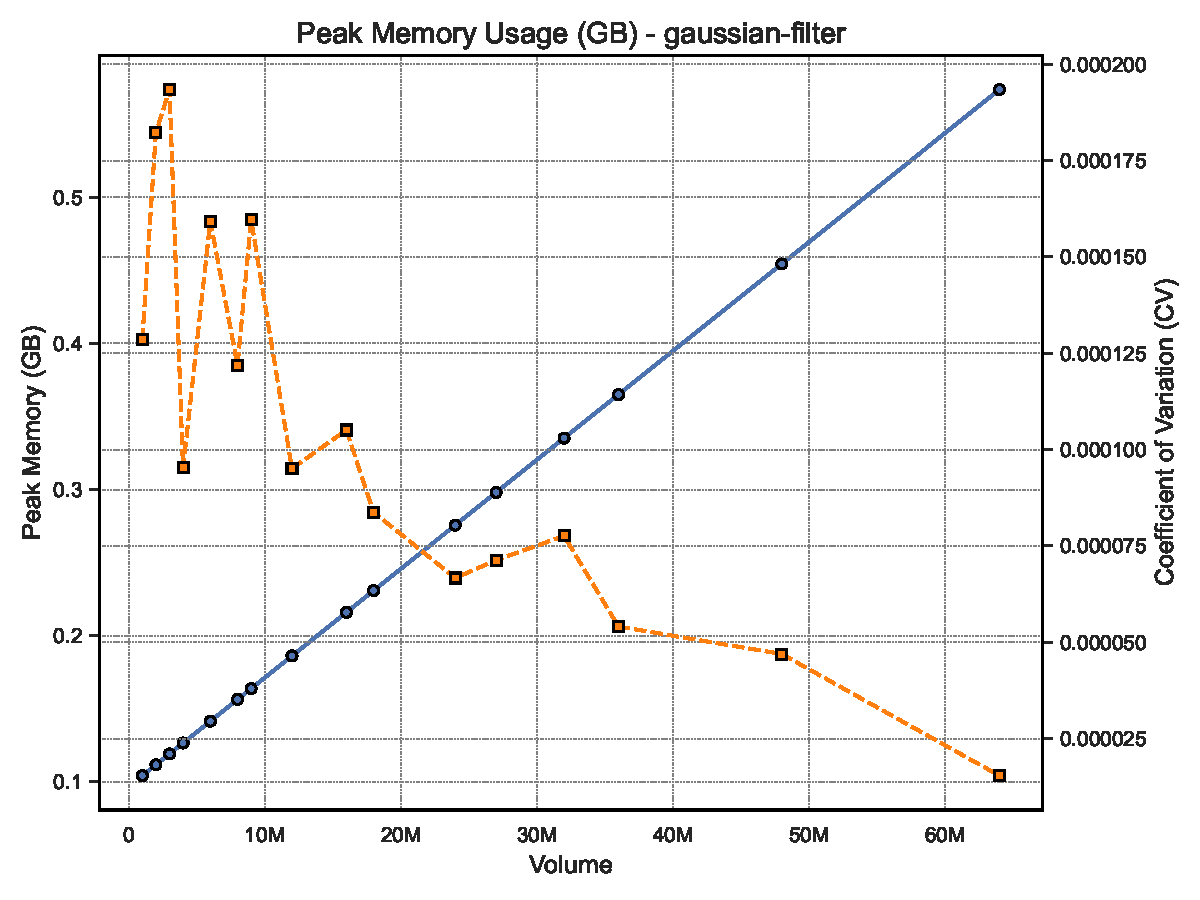
\includegraphics[width=\textwidth]{assets/images/05/peak_memory_by_volume_gaussian-filter}
        \caption{Gaussian Filter: Memory consumption scales linearly,
            though less steeply than \ac{GST3D}.}
    \end{subfigure}
    \caption{Peak memory usage by volume for three operators: Envelope, \ac{GST3D}, and the Gaussian Filter.
    Memory usage grows linearly with volume, with larger volumes requiring more resources.}
    \label{fig:peak_memory_facet}
\end{figure*}

Figure~\ref{fig:ex_peak_mu_facet} indicate that execution time and memory usage both rise in near-linear fashion across all operators.
Similarly, figure~\ref{fig:execution_time_by_volume_facet} confirm that execution time correlates strongly with volume for each seismic algorithm evaluated.

\begin{figure*}[htbp]
    \centering
    \begin{subfigure}[t]{0.49\textwidth}
        \centering
        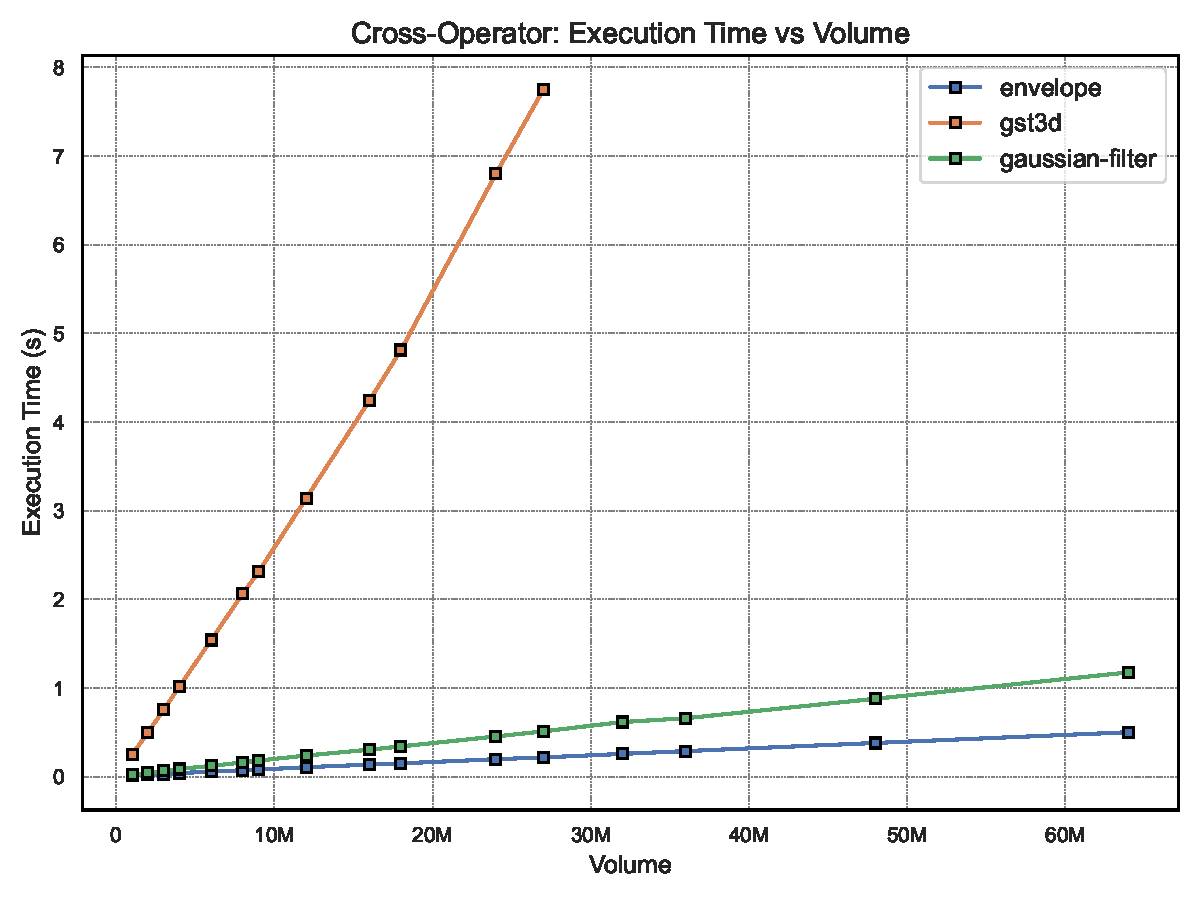
\includegraphics[width=\textwidth]{assets/images/05/cross_execution_time_by_volume}
        \caption{Execution time by volume for Envelope, \ac{GST3D}, and the Gaussian Filter.}
    \end{subfigure}
    \hfill
    \begin{subfigure}[t]{0.49\textwidth}
        \centering
        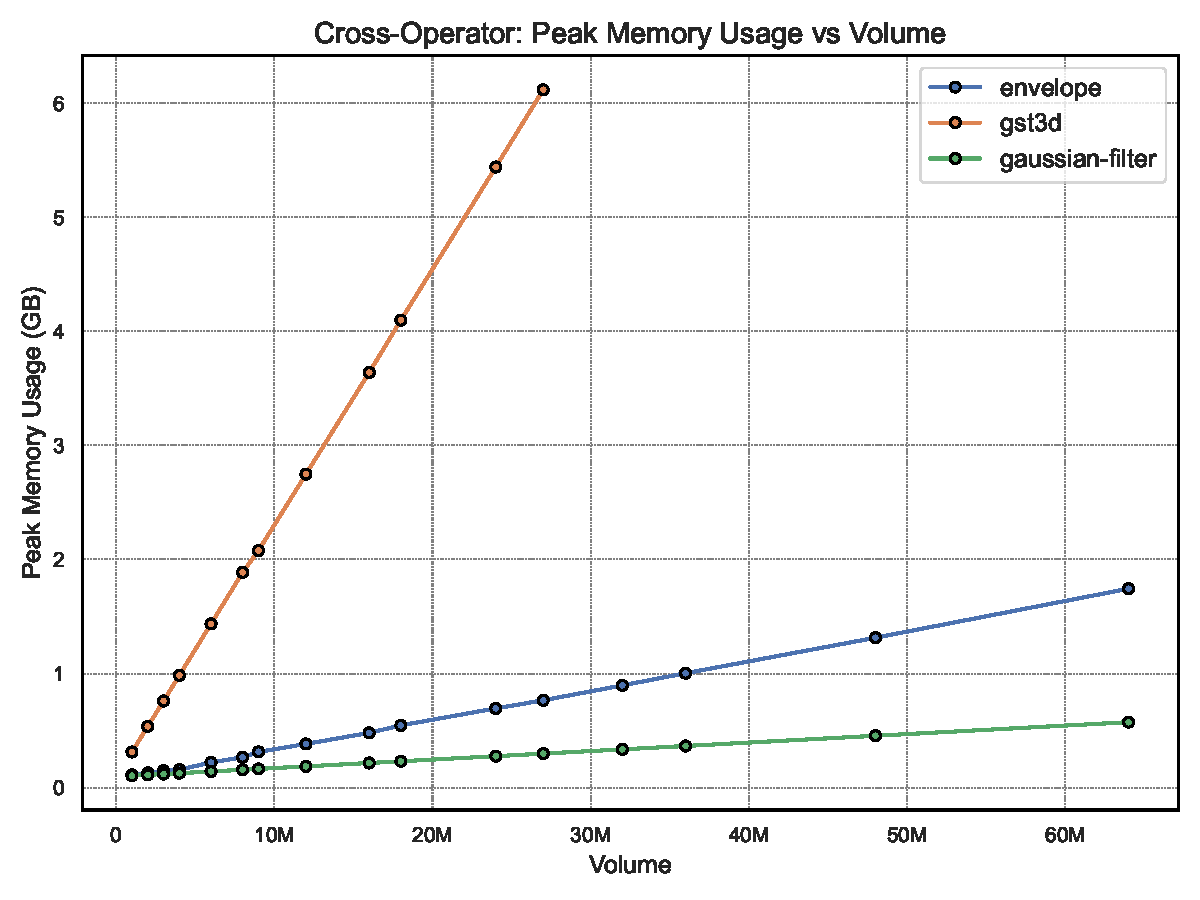
\includegraphics[width=\textwidth]{assets/images/05/cross_peak_memory_by_volume}
        \caption{Peak memory usage by volume for Envelope, \ac{GST3D}, and the Gaussian Filter.}
    \end{subfigure}
    \hfill
    \begin{subfigure}[t]{0.49\textwidth}
        \centering
        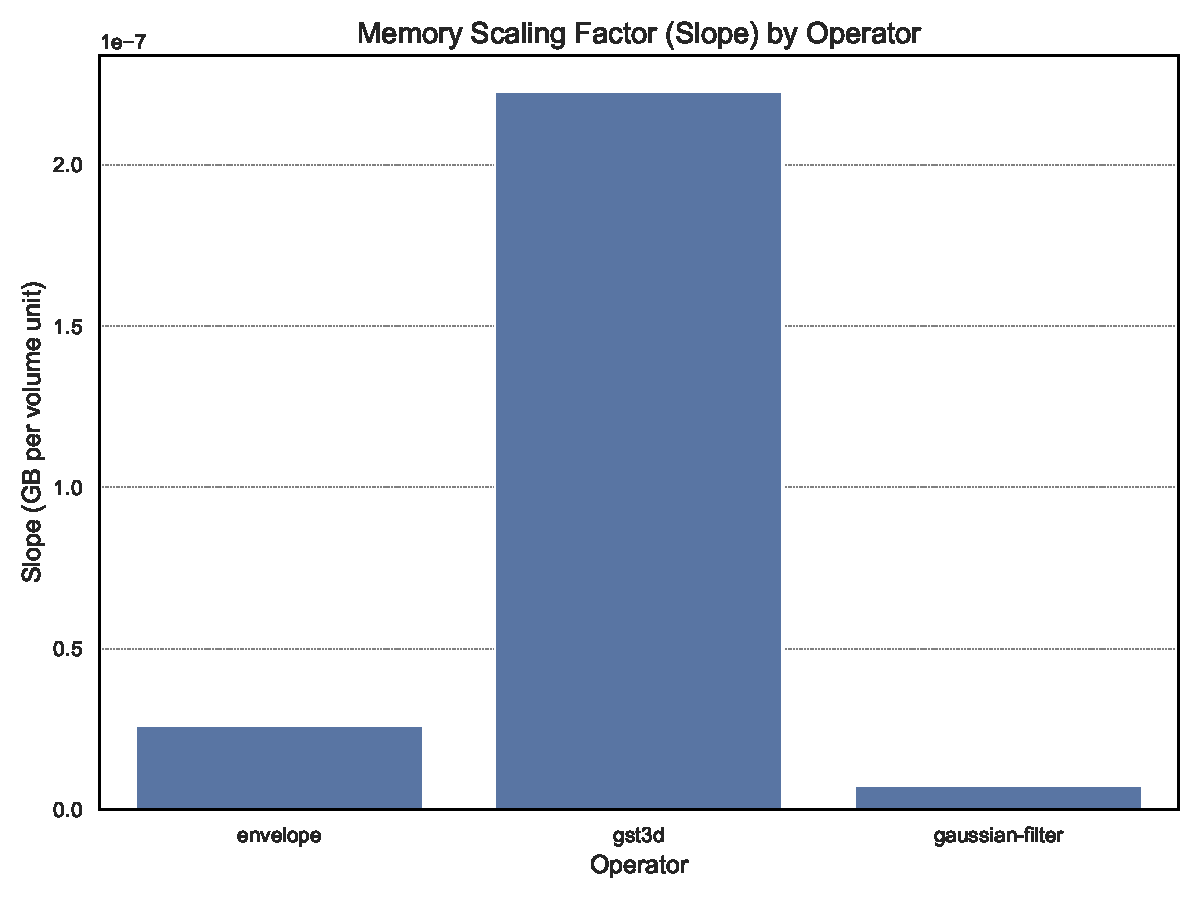
\includegraphics[width=\textwidth]{assets/images/05/cross_operator_memory_scaling_factor}
        \caption{Linear-fit slope of memory usage vs volume by operator.
        Higher values imply more rapid growth with increasing volume.}
    \end{subfigure}
    \caption{Peak memory usage and execution time by volume for Envelope, \ac{GST3D}, and the Gaussian Filter.
    Both metrics exhibit a clear linear trend, with larger volumes requiring more resources.}
    \label{fig:ex_peak_mu_facet}
\end{figure*}

\begin{figure*}[htbp]
    \centering
    \begin{subfigure}[t]{0.49\textwidth}
        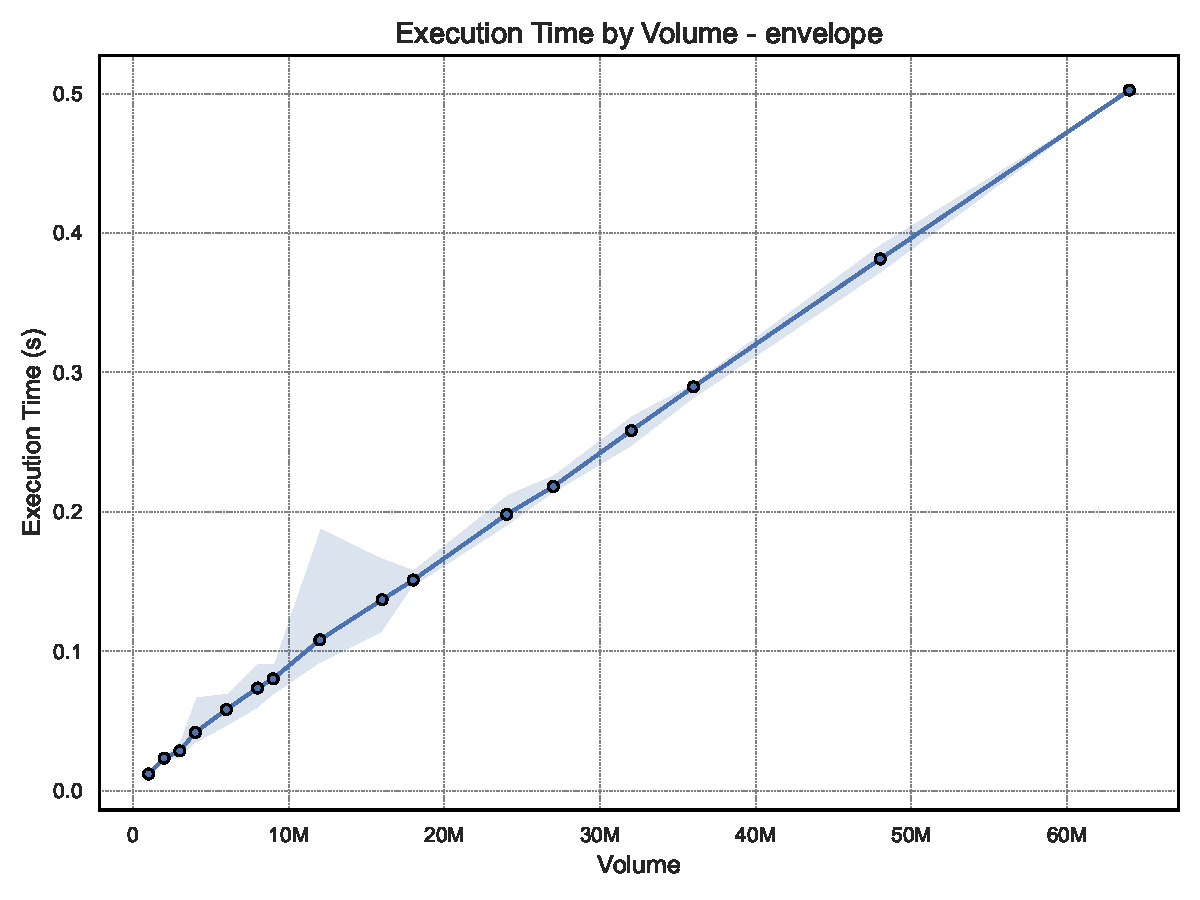
\includegraphics[width=\textwidth]{assets/images/05/execution_time_by_volume_envelope}
    \end{subfigure}
    \hfill
    \begin{subfigure}[t]{0.49\textwidth}
        \centering
        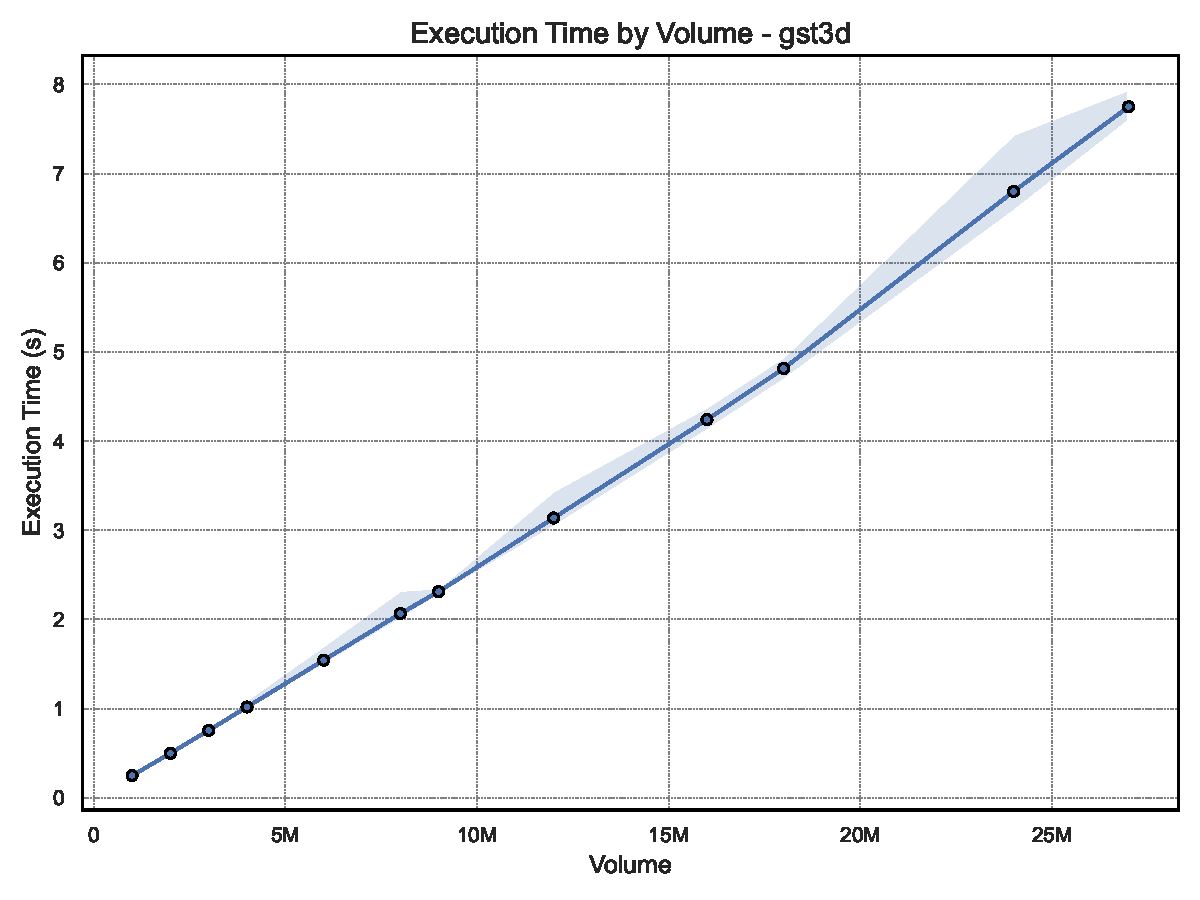
\includegraphics[width=\textwidth]{assets/images/05/execution_time_by_volume_gst3d}
    \end{subfigure}
    \hfill
    \begin{subfigure}[t]{0.49\textwidth}
        \centering
        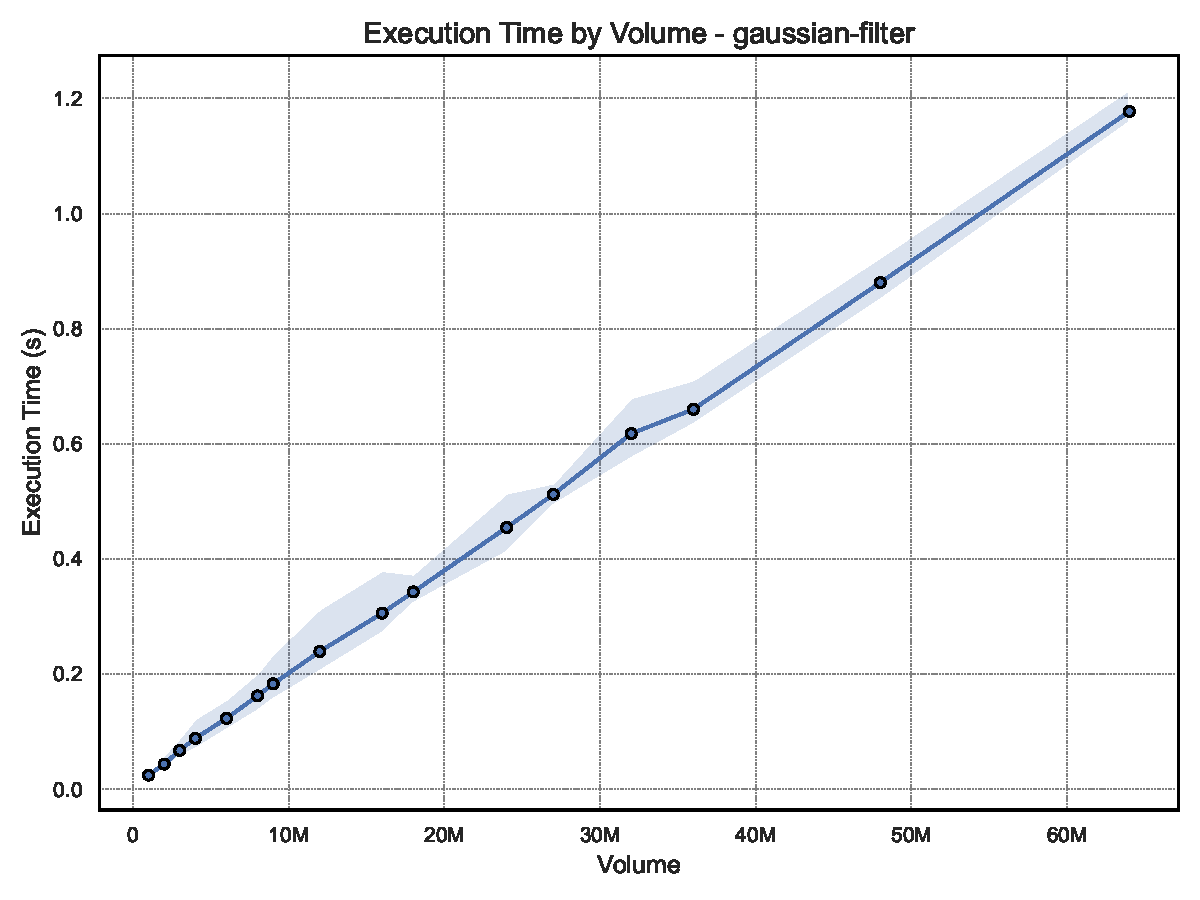
\includegraphics[width=\textwidth]{assets/images/05/execution_time_by_volume_gaussian-filter}
    \end{subfigure}
    \caption{Execution time by volume for Envelope, \ac{GST3D}, and the Gaussian Filter.
    The chart shows a clear linear trend, with larger volumes requiring more time to process.}
    \label{fig:execution_time_by_volume_facet}
\end{figure*}

\subsection{Execution Time Distributions and Scaling Factor}
\label{subsec:execution-time-distributions-and-scaling}

Figure~\ref{fig:execution_time_distribution_facet} depict right-skewed distributions of run durations, indicative of gamma- or lognormal-like behavior.
Most runs complete quickly, but outliers at the high end extend the tail.

\begin{figure*}[htbp]
    \centering
    \begin{subfigure}[t]{0.49\textwidth}
        \centering
        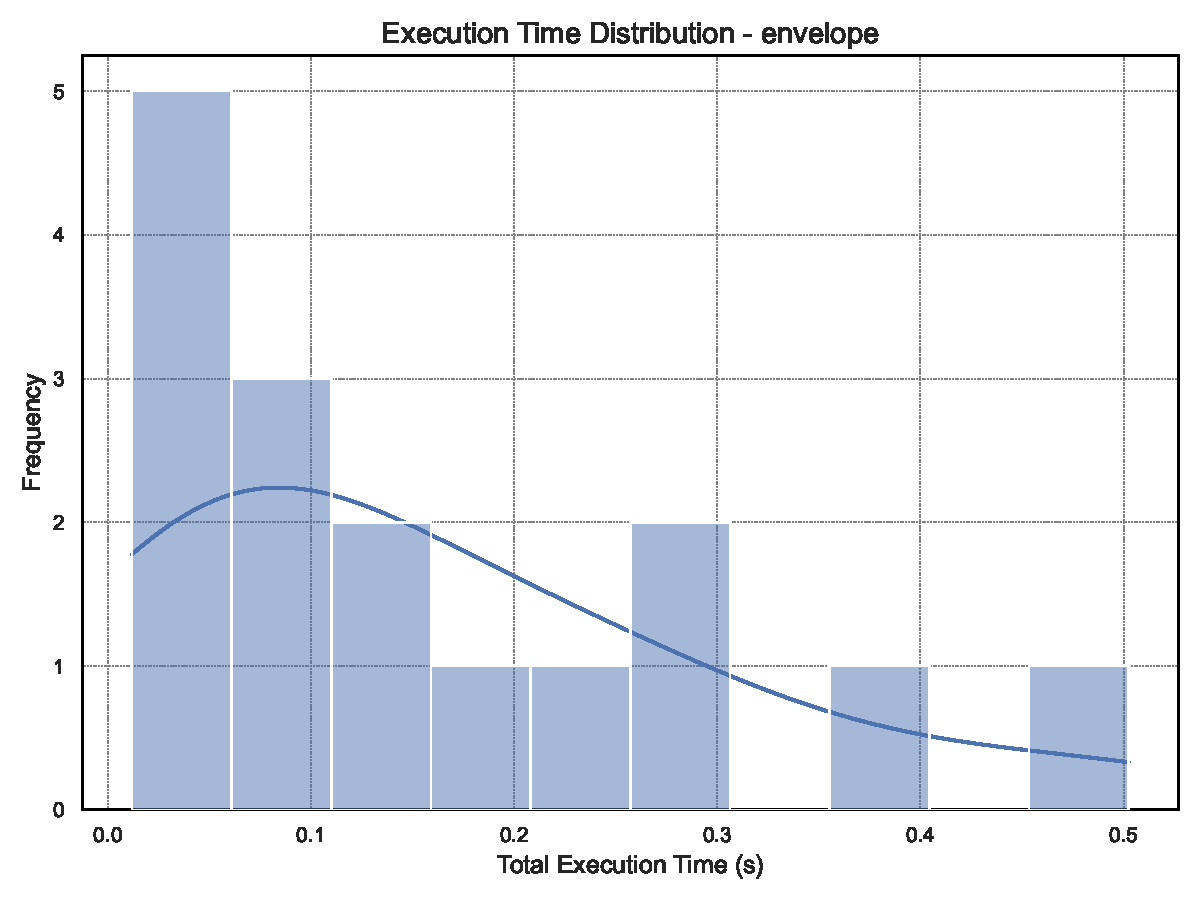
\includegraphics[width=\textwidth]{assets/images/05/execution_time_distribution_envelope}
    \end{subfigure}
    \hfill
    \begin{subfigure}[t]{0.49\textwidth}
        \centering
        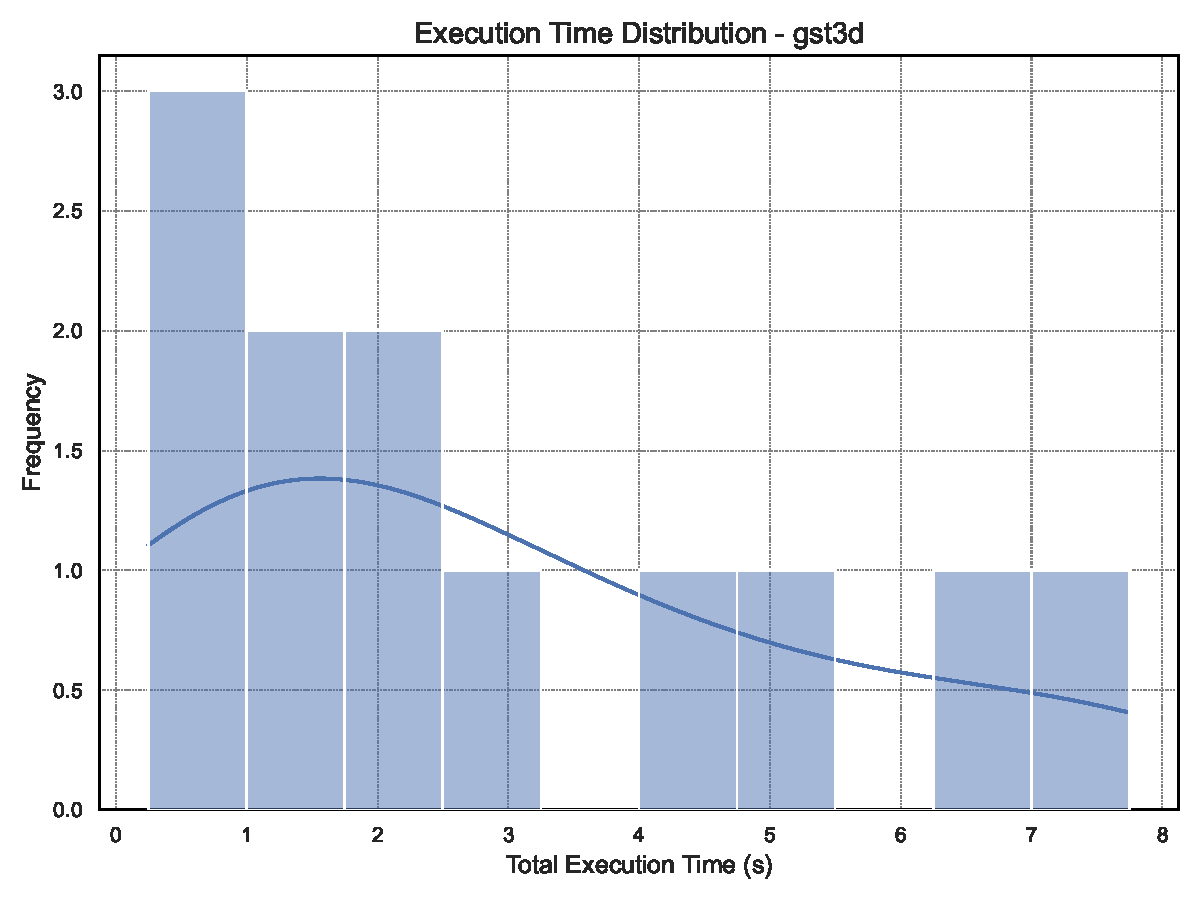
\includegraphics[width=\textwidth]{assets/images/05/execution_time_distribution_gst3d}
    \end{subfigure}
    \hfill
    \begin{subfigure}[t]{0.49\textwidth}
        \centering
        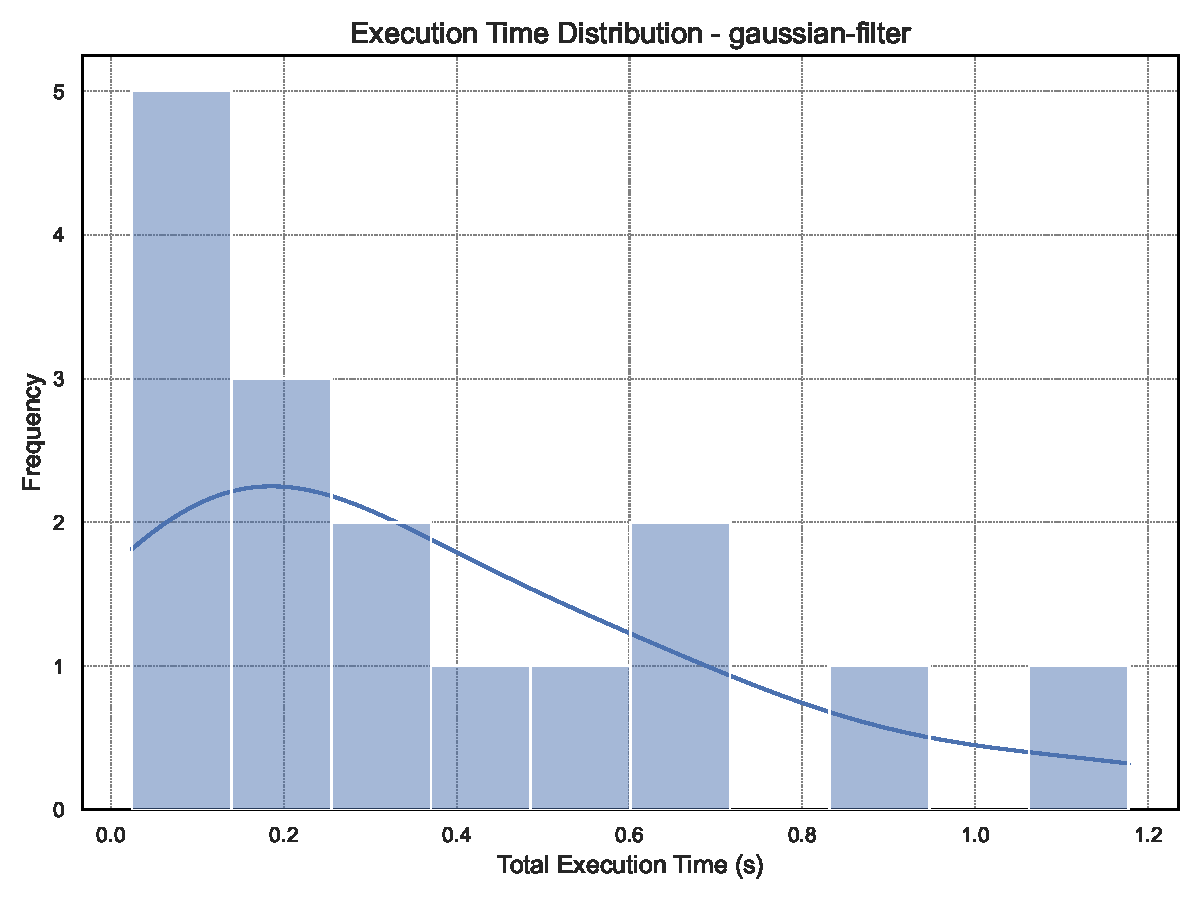
\includegraphics[width=\textwidth]{assets/images/05/execution_time_distribution_gaussian-filter}
    \end{subfigure}
    \caption{Execution time distributions for Envelope, \ac{GST3D}, and the Gaussian Filter.
    The distribution shows a clear left skew, with most runs completing quickly.}
    \label{fig:execution_time_distribution_facet}
\end{figure*}

Figure~\ref{fig:ex_peak_mu_facet} shows a bar chart of the linear-fit coefficients (slopes) for each operator’s average peak \ac{RAM} usage vs volume.
\ac{GST3D} exhibits the largest slope, reflecting more elaborate data structures and intermediate buffers for discontinuity detection.
Envelope has a moderate slope, whereas Gaussian Filter is the least steep, indicating more incremental memory use.

\subsection{Dimension-Specific and Time-Progression Analysis}
\label{subsec:dimension-specific-and-time-progression-analysis}

Figure~\ref{fig:memory_usage_by_configuration_envelope} show dimension-specific breakdowns (inlines, xlines, samples) for the Envelope operator, confirming that each dimension contributes similarly to overall memory usage.
Also, figure~\ref{fig:memory_usage_by_configuration_envelope} illustrate that higher memory consumption correlates with longer run durations for the Envelope operator.

\begin{figure*}[htbp]
    \centering
    \begin{subfigure}[t]{0.49\textwidth}
        \centering
        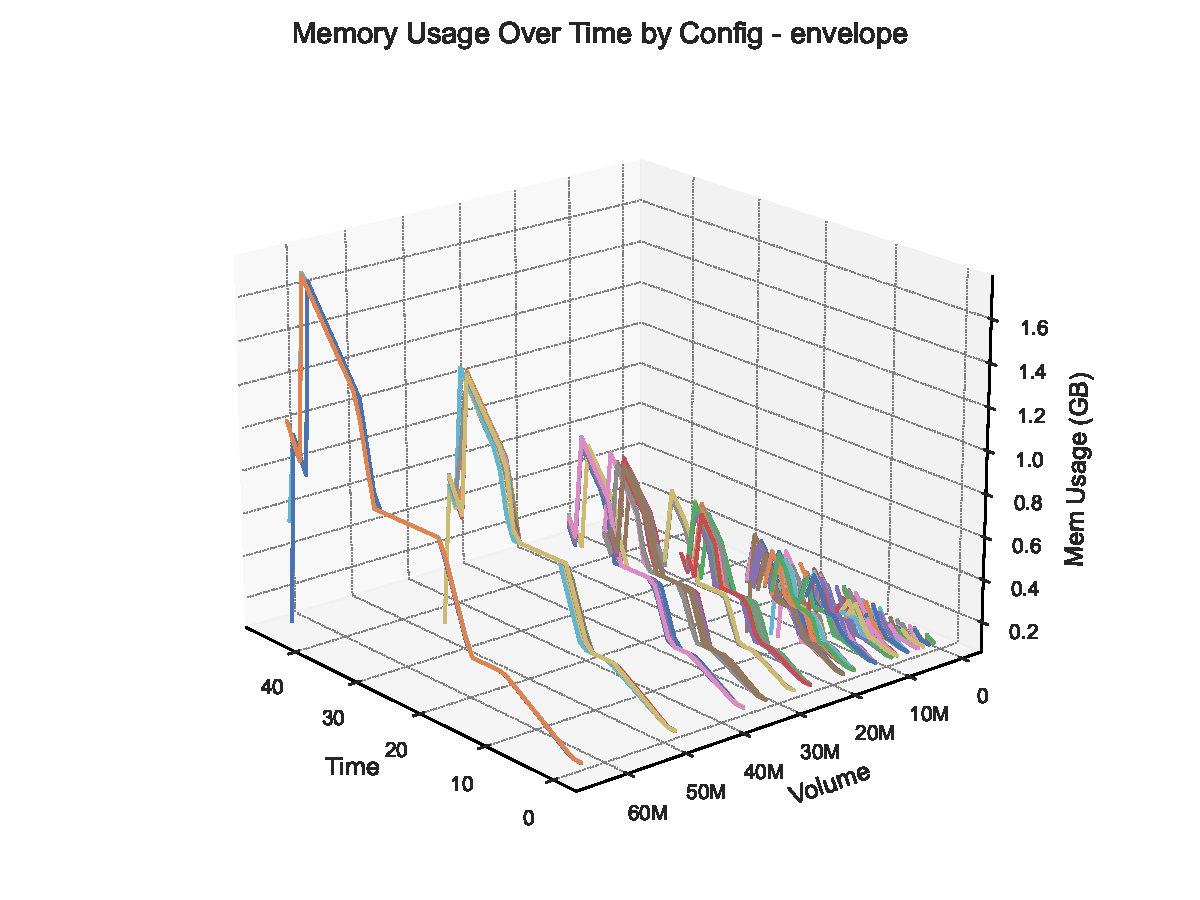
\includegraphics[width=\textwidth]{assets/images/05/memory_usage_by_configuration_envelope}
        \caption{Memory usage by inlines, xlines, and samples for Envelope.
        All dimensions contribute equally to memory consumption.}
    \end{subfigure}
    \hfill
    \begin{subfigure}[t]{0.49\textwidth}
        \centering
        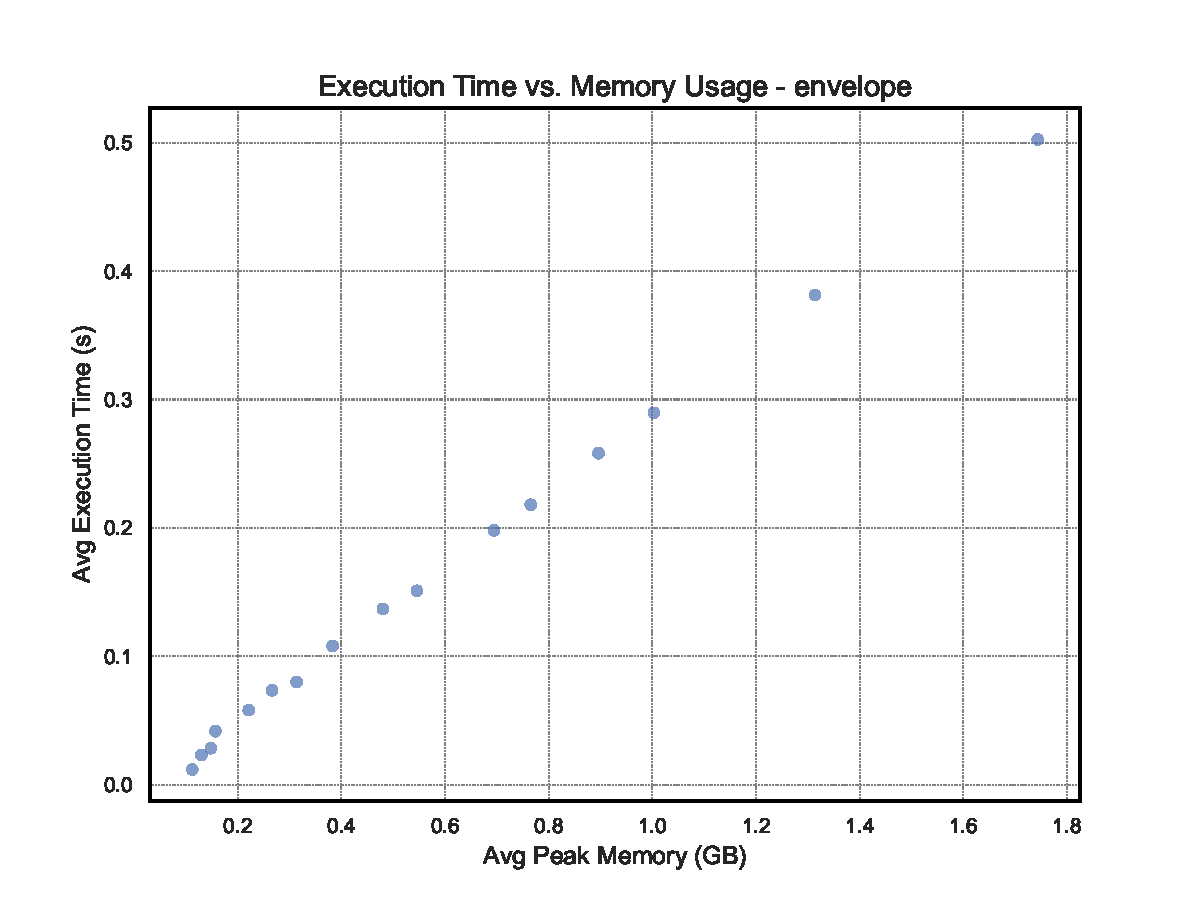
\includegraphics[width=\textwidth]{assets/images/05/execution_time_vs_memory_envelope}
        \caption{Execution time vs memory usage for Envelope.}
    \end{subfigure}
    \hfill
    \begin{subfigure}[t]{0.49\textwidth}
        \centering
        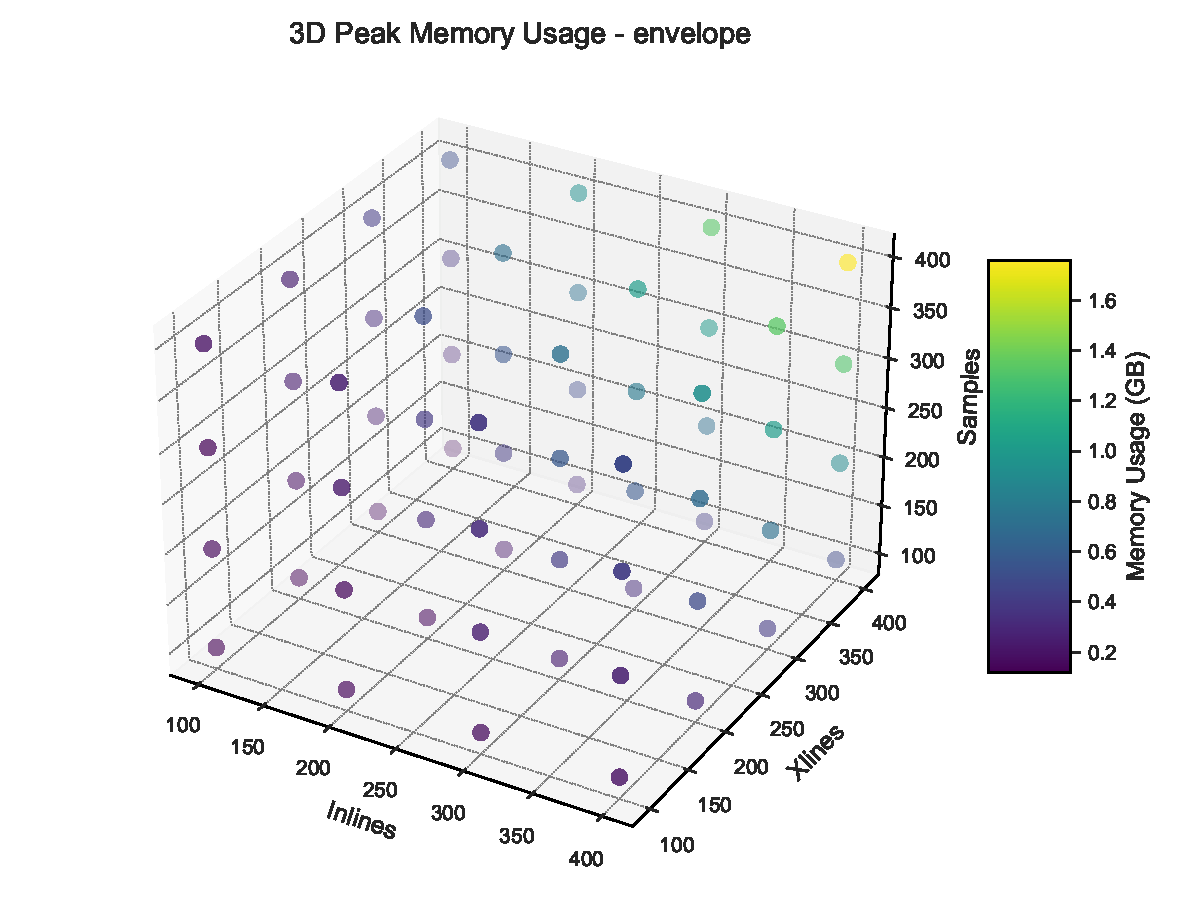
\includegraphics[width=\textwidth]{assets/images/05/memory_usage_inlines_xlines_samples_heatmap_envelope}
        \caption{Memory usage heatmap by inlines, xlines, and samples for Envelope.}
    \end{subfigure}
    \caption{Memory usage and execution time analysis for the Envelope operator.}
    \label{fig:memory_usage_by_configuration_envelope}
\end{figure*}

Violin charts in Figure~\ref{fig:memory_usage_distribution} illustrate memory usage fluctuations over time for each operator.
Envelope shows wider distributions, indicating more gradual ramps and fluctuations.
Gaussian Filter and \ac{GST3D} reach stable peak memory usage more rapidly, resulting in thinner violins.

\begin{figure*}[htbp]
    \centering
    \begin{subfigure}[t]{0.49\textwidth}
        \centering
        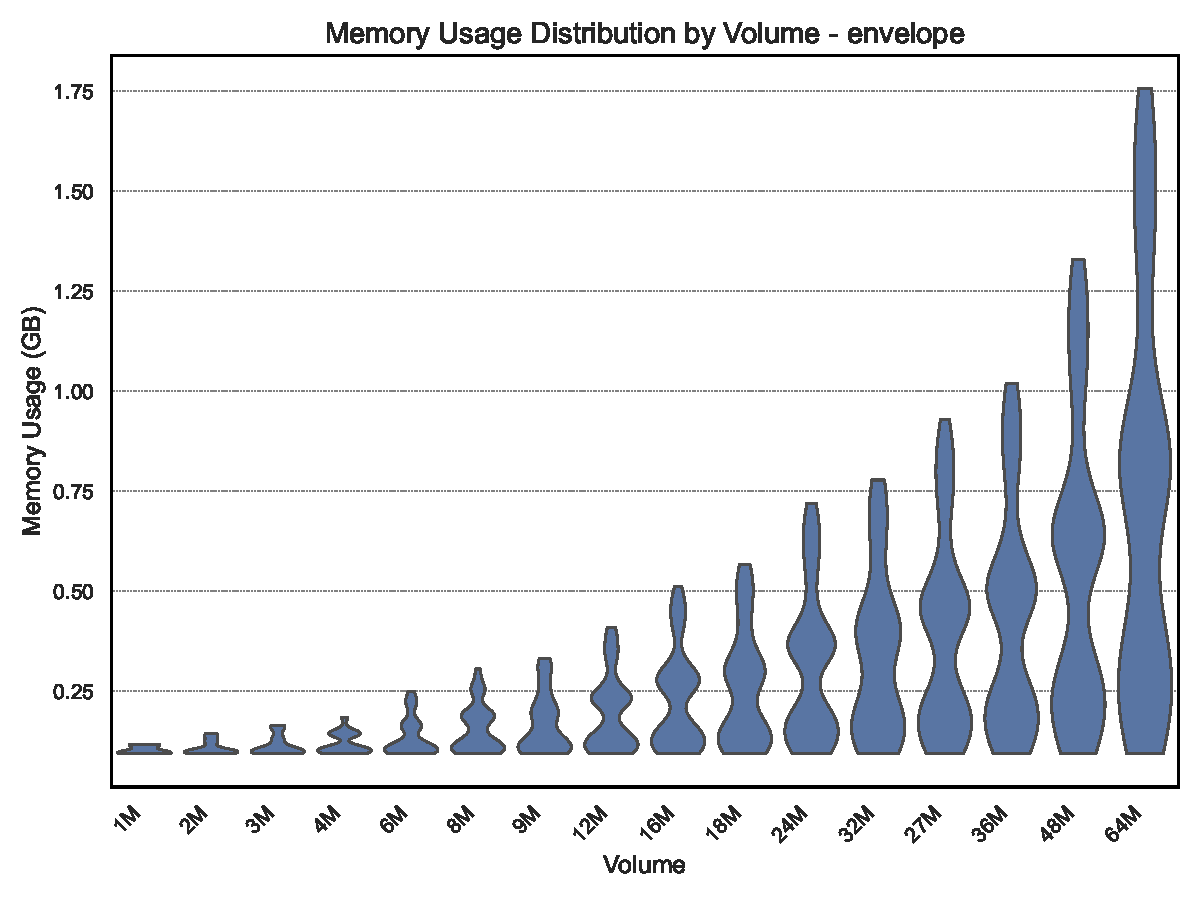
\includegraphics[width=\textwidth]{assets/images/05/memory_usage_distribution_envelope}
    \end{subfigure}
    \hfill
    \begin{subfigure}[t]{0.49\textwidth}
        \centering
        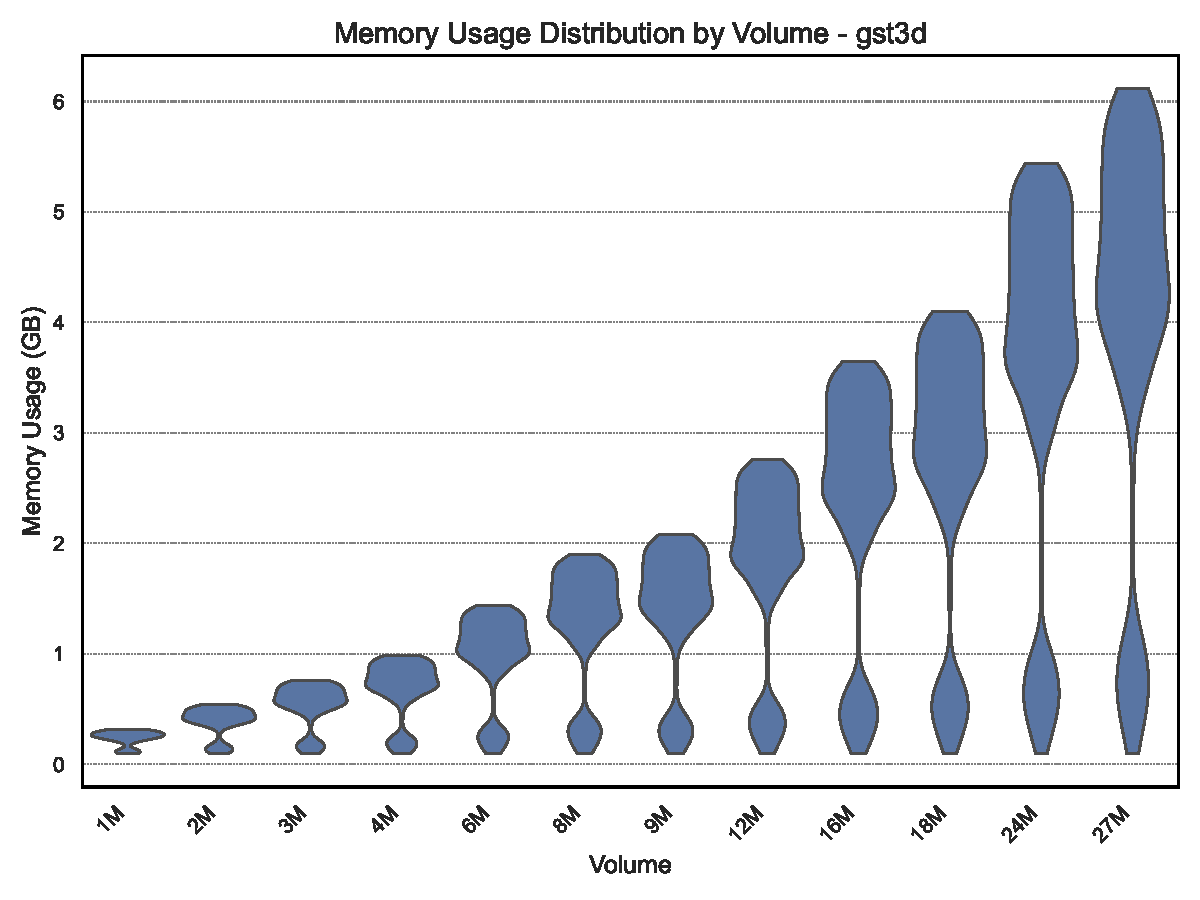
\includegraphics[width=\textwidth]{assets/images/05/memory_usage_distribution_gst3d}
    \end{subfigure}
    \hfill
    \begin{subfigure}[t]{0.49\textwidth}
        \centering
        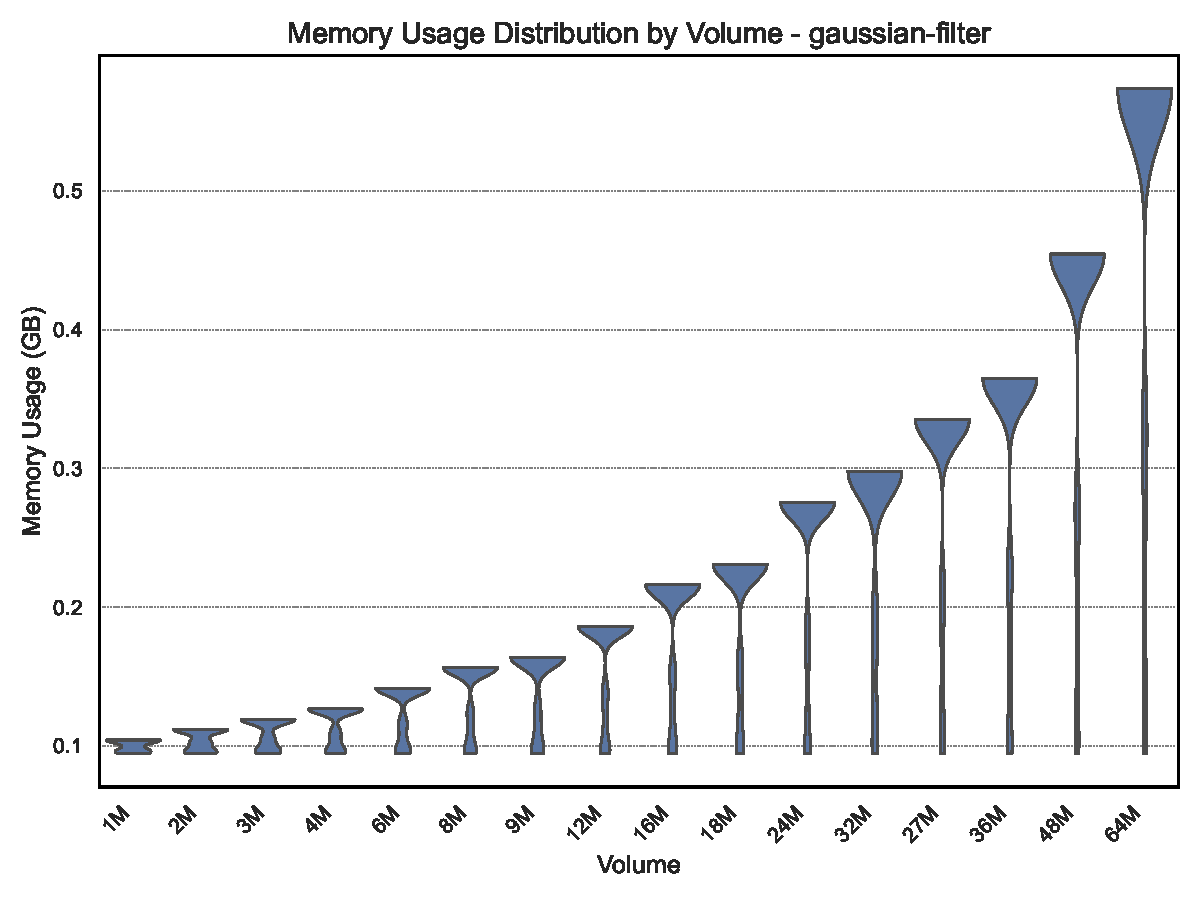
\includegraphics[width=\textwidth]{assets/images/05/memory_usage_distribution_gaussian-filter}
    \end{subfigure}
    \caption{Violin charts of memory usage over time for Envelope, \ac{GST3D}, and the Gaussian Filter.
    Envelope exhibits wider distributions, while \ac{GST3D} and the Gaussian Filter show more stable memory usage.}
    \label{fig:memory_usage_distribution}
\end{figure*}

Figure~\ref{fig:memory_usage_by_configuration_envelope} shows a heatmap indicating that memory usage rises uniformly across the three dimensions.
Figure~\ref{fig:inline_xline_memory_usage_progression_envelope} confirm that Envelope ramps more uniformly in time.

\begin{figure}[htbp]
    \centering
    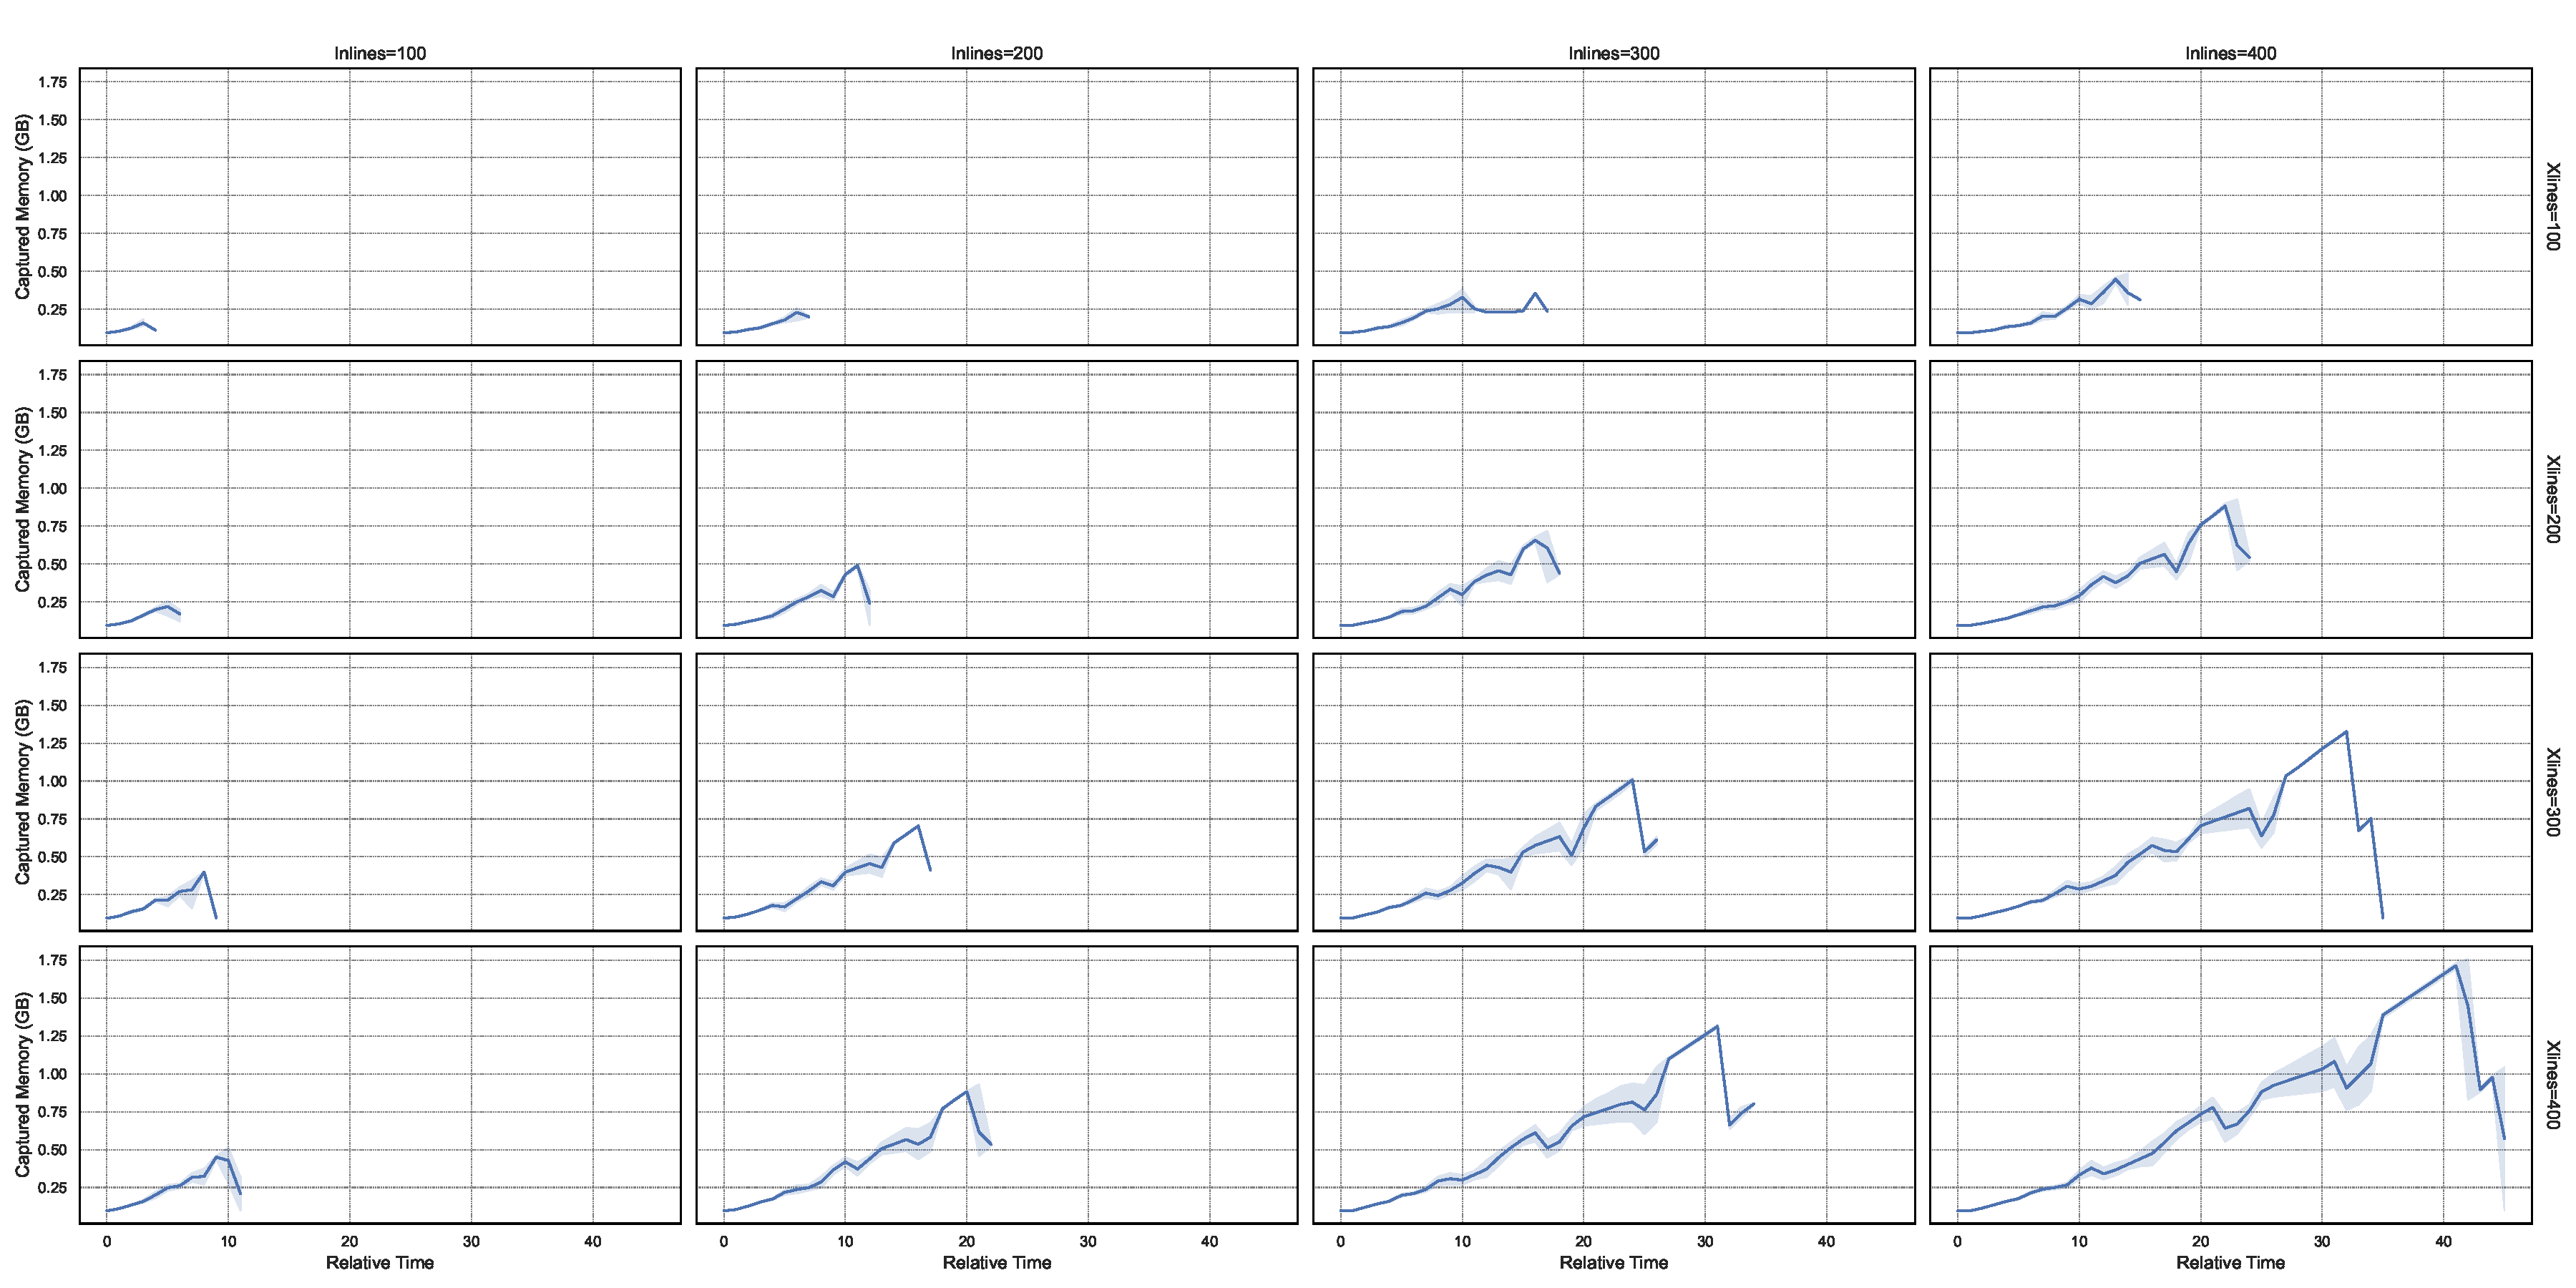
\includegraphics[width=\textwidth]{assets/images/05/inline_xline_memory_usage_progression_envelope}
    \caption{Memory usage progression by inlines and xlines for Envelope.}
    \label{fig:inline_xline_memory_usage_progression_envelope}
\end{figure}

\subsection{Memory Safety Margins}
\label{subsec:memory-safety-margins}

Figure~\ref{fig:memory_safety_margins} highlight the difference between average and 95th-percentile memory usage across tested volumes.
Envelope and \ac{GST3D} can exhibit large gaps in memory usage, which indicates that some runs exceed the typical allocation by a significant margin.
Isolating experiments via containerization did not fully eliminate kernel-level optimizations or other system effects that cause these outliers.

\begin{figure*}[htbp]
    \centering
    \begin{subfigure}[t]{0.49\textwidth}
        \centering
        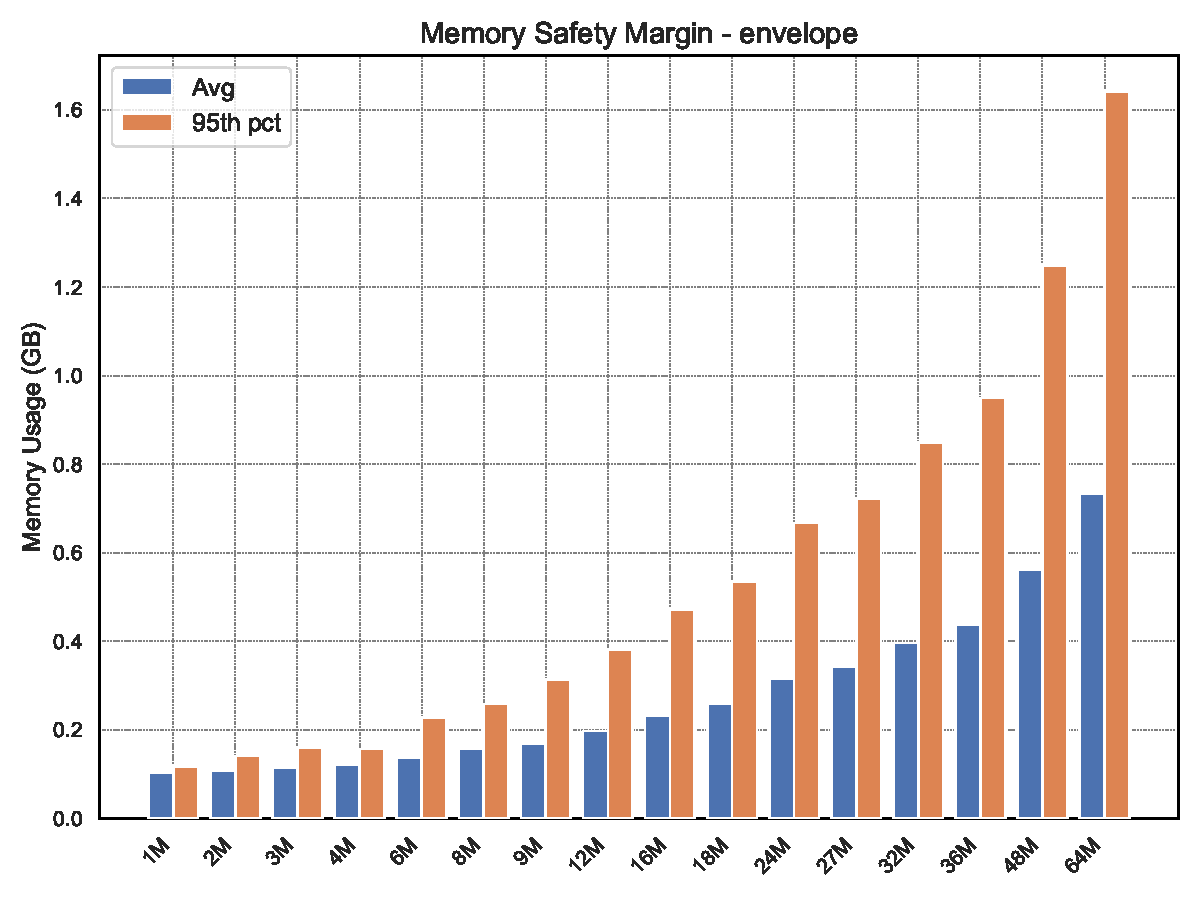
\includegraphics[width=\textwidth]{assets/images/05/memory_safety_margin_envelope}
    \end{subfigure}
    \hfill
    \begin{subfigure}[t]{0.49\textwidth}
        \centering
        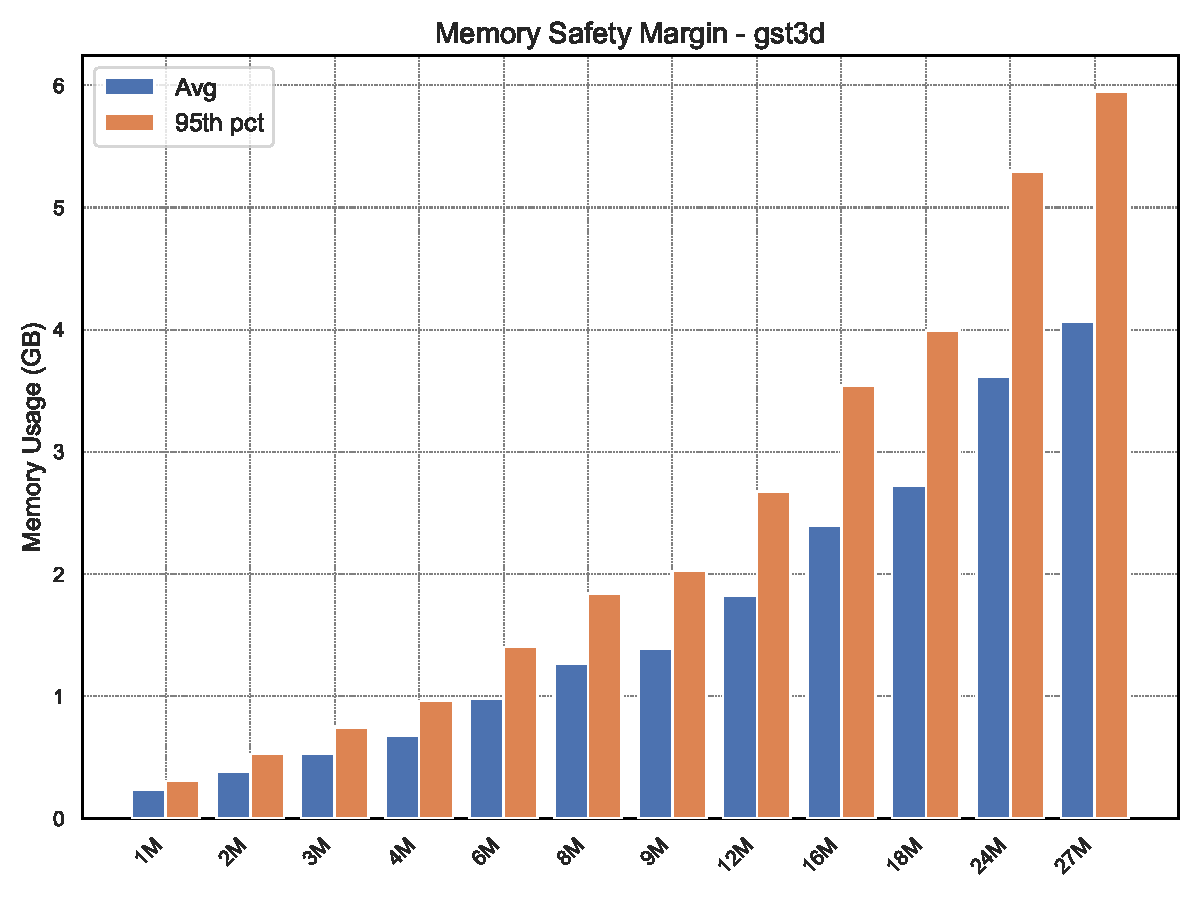
\includegraphics[width=\textwidth]{assets/images/05/memory_safety_margin_gst3d}
    \end{subfigure}
    \hfill
    \begin{subfigure}[t]{0.49\textwidth}
        \centering
        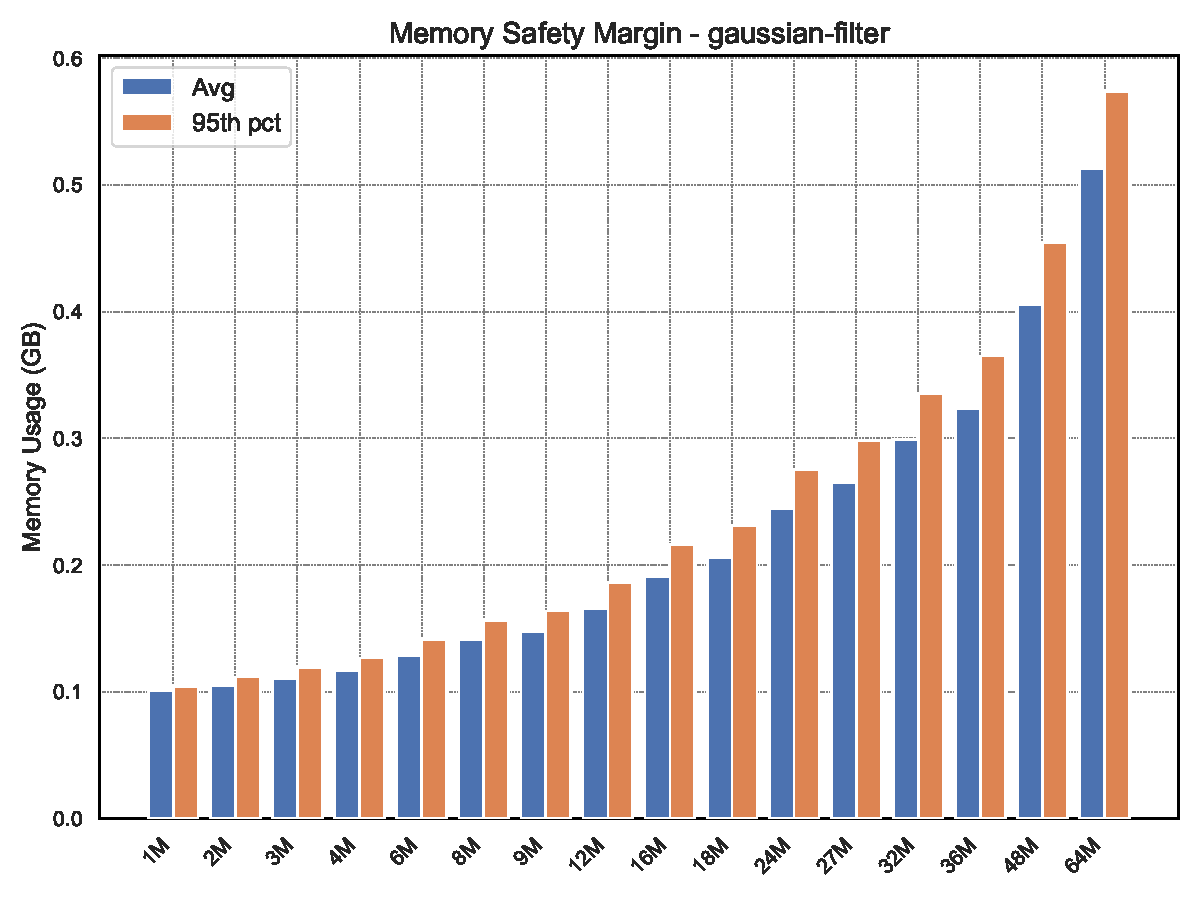
\includegraphics[width=\textwidth]{assets/images/05/memory_safety_margin_gaussian-filter}
    \end{subfigure}
    \caption{Memory safety margins for Envelope, \ac{GST3D}, and the Gaussian Filter.
    The 95th percentile often surpasses the average, suggesting occasional high-memory runs.}
    \label{fig:memory_safety_margin}
\end{figure*}

\subsection{Dimension Correlations}
\label{subsec:dimension-correlations}

Figure~\ref{fig:memory_vs_dimensions_pairplot_gst3d} presents a pairplot examining \ac{GST3D} memory usage alongside inlines, xlines, and samples.
Positive slopes confirm that higher dimensions correlate with increased memory.
Negative slopes among dimension--dimension cells primarily reflect the experimental test grid, where large values in one dimension often paired with smaller values in another.
Despite these trade-offs, the net memory footprint rose whenever any dimension increased significantly.

\begin{figure}[htbp]
    \centering
    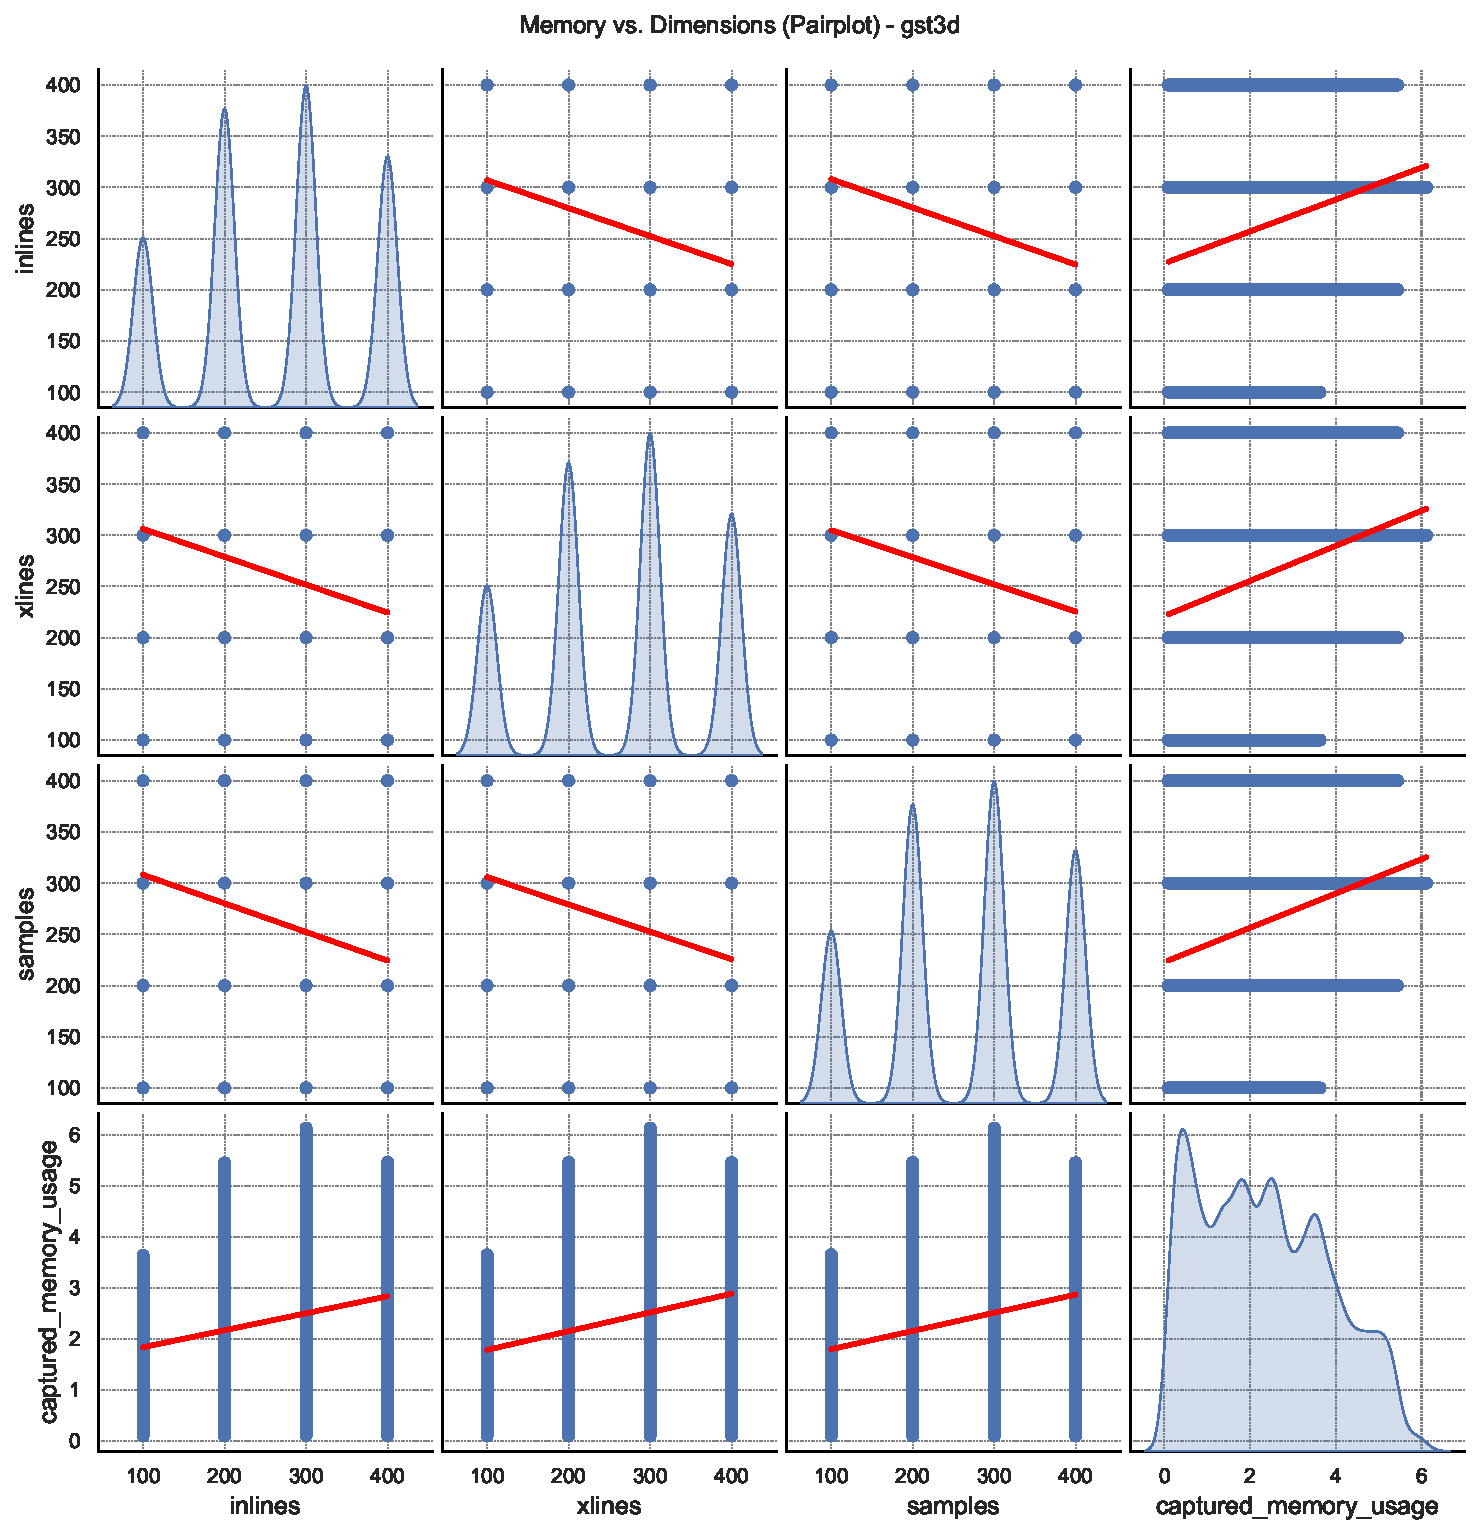
\includegraphics[width=0.9\textwidth]{assets/images/05/memory_vs_dimensions_pairplot_gst3d}
    \caption{Pairplot of memory usage vs inlines, xlines, and samples for \ac{GST3D}.
    Larger shapes yield higher \ac{RAM} usage.}
    \label{fig:memory_vs_dimensions_pairplot_gst3d}
\end{figure}

\subsection{Summary of Observed Resource Usage}
\label{subsec:resource-usage-summary}

Table~\ref{tab:operator_summary_aggregates} summarizes key metrics for each operator, including tested volume ranges, peak memory usage ranges, and execution time ranges.
It combines the raw data into concise statistics that highlight how quickly memory usage and runtime escalate with increasing volume.

\begin{table}[htbp]
    \centering
    \begin{tabular}{lcccc}
        \hline
        \textbf{Operator} & \textbf{Volume Range} & \textbf{Peak Mem. Usage (GB)} & \textbf{Exec. Time (s)} \\ \hline
        Envelope &
        $10^6 \!\to\! 6.4\times10^7$ &
        0.10 -- 1.76 &
        0.0106 -- 0.5025 \\
        \ac{GST3D} &
        $10^6 \!\to\! 2.7\times10^7$ &
        0.31 -- 6.12 &
        0.2475 -- 7.75 \\
        Gaussian Filter &
        $10^6 \!\to\! 6.4\times10^7$ &
        0.10 -- 0.57 &
        0.0232 -- 1.22 \\
        \hline
    \end{tabular}
    \caption{Resource usage summary for Envelope, \ac{GST3D}, and Gaussian Filter.
    Volumes are specified in number of samples (e.g., $1000000$ = $10^6$).
    Memory usage values appear in GB, and times appear in seconds.
    Each range denotes the minimum and maximum observed across tested volumes.}
    \label{tab:operator_summary_aggregates}
\end{table}

Table~\ref{tab:operator_summary_aggregates} confirms that \ac{GST3D} consistently displays the highest memory usage for similarly sized volumes, with Envelope at an intermediate level, and the Gaussian Filter at a lower bound, though it still scales markedly with volume.
Overall, both memory and execution time exhibit near-linear growth, reinforcing the importance of volume-driven resource estimation.
These findings guide \ac{HPC} users to anticipate how large seismic datasets will stress system \ac{RAM} and runtime allocations, especially in scenarios with competing workloads.


\section{Model Performance Overview}
\label{sec:pmc-results-model-performance-overview}

%- chart assets/images/05/actual_vs_predicted_by_model.pdf shows the results per model and operator. It compares the actual and predicted values. It is clear that most of the models got a pretty good result, but a few of those we can highlight. Namely linear regression,xgboost,and elastic net went pretty well for all models
%- chart assets/images/05/residual_vs_predicted.pdf shows clearly that most models got pretty low residuals. Really close to 0. A few models for a few operators went pretty bad, specially for the gst3d operator
%- chart assets/images/05/cross_model_r2_bar.pdf shows all models r2 scores per operator. We can see that the neural network was the only that perform poorly on gst3d, and we can corroborate the results from the previous chart, that the linear regression, xgboost, and elastic net were the best models
%- charts assets/images/05/score_by_model_envelope.pdf, assets/images/05/score_by_model_gst3d.pdf, assets/images/05/score_by_model_gaussian_filter.pdf show the score for each model per operator. We can see that the best model varies depending on the operator, but we have many models that are really close. For envelope the best model was gradient boost, with a score of 2,579 while for gaussian filter many models performed well, being linear regression the best with a score of 2,904. For gst3d the top score was 2,970 for the decision tree model
%- chart assets/images/05/best_model_per_operator.pdf shows that in a single chart (what was mentioned above)


\section{Feature Selection Experiments}
\label{sec:pmc-results-feature-selection-experiments}


\section{Data Reduction Studies}
\label{sec:pmc-results-data-reduction-studies}


\section{Summary of Findings}
\label{sec:pmc-results-summary-of-findings}